%!TEX root = ../thesis.tex
\chapter{Results and Discussion}
\label{ch:results}

\section{Quantitative Analysis}

For evaluating the performance of the model on unseen images we use the photobox test set, comprising 50 labeled images. The model only detects up to 300 colonies, so all metrics are calculated with 300 as the upper boundary for ground truth boxes.

An IoU (intersection over union) of 0.5 was chosen for deciding between true and false positives. As seen in Figure \ref{fig:ious}, an IoU of 0.5 requires a quite clear overlap in both boxes to count as a correct prediction, but is also not too strict, because accurate counting is more important than precise localisation.

\begin{figure}[hbt]
  \centering
  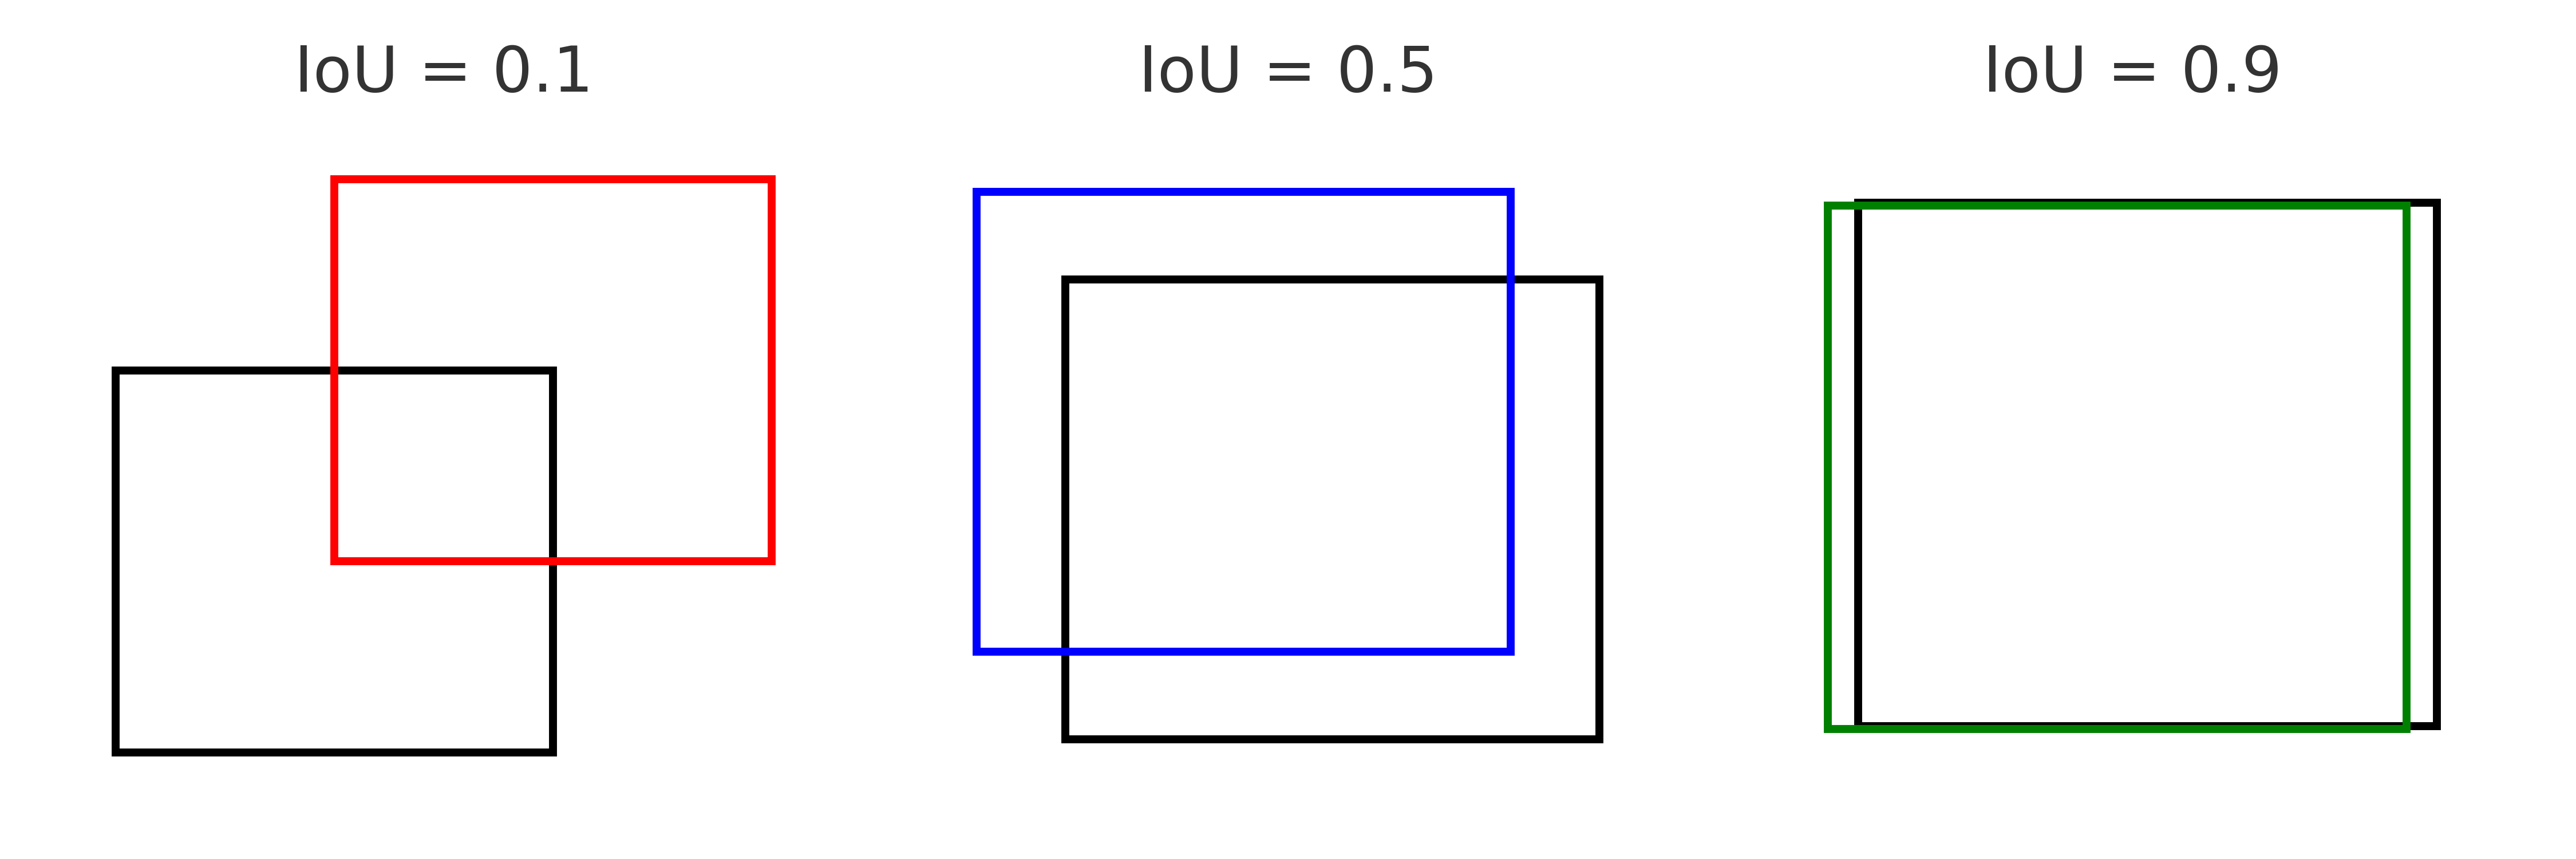
\includegraphics[width=0.8\textwidth]{assets/ious.png}
  \caption{Examples of IoU values}
  \label{fig:ious}
\end{figure}

Of all the 1,924 found boxes on the test set, \textbf{92.9\%} were in fact colonies (precision over all boxes in test set). Also \textbf{87.3\%} of the 2,145 boxes present in the labels of the test set were predicted (recall over all boxes in test set). The mean absolute error for counting the test set is \textbf{6.26}, the sMAPE is \textbf{0.153}.

When taking a mean over the individual precision and recall values for each of the 50 images in the test set, mean precision is 78.1\% and mean recall is 90.1\% (this is \textit{not} related to the mAP metric used earlier). Interestingly, when taking these values while including only images that contain 2 or more colonies, mean precision is 86.6\%. This shows that false positives on empty dishes are a problem. When taking only images with more than 50 colonies into account, mean precision rises to 97.7\%, which shows that false positives almost never occur for images with higher numbers of colonies.

This is trend is also visible in Figure \ref{fig:counting_test}. The model counts too many colonies for low colony counts (lower precision) but too few for images with more colonies (lower recall). The outlier seen in the chart is image Figure \ref{fig:test_outlier}, where only 187 of 398 colonies are detected. This shows the model has significant recall problems for large colony counts.

\begin{figure}
     \centering
     \begin{subfigure}[b]{0.45\textwidth}
         \centering
         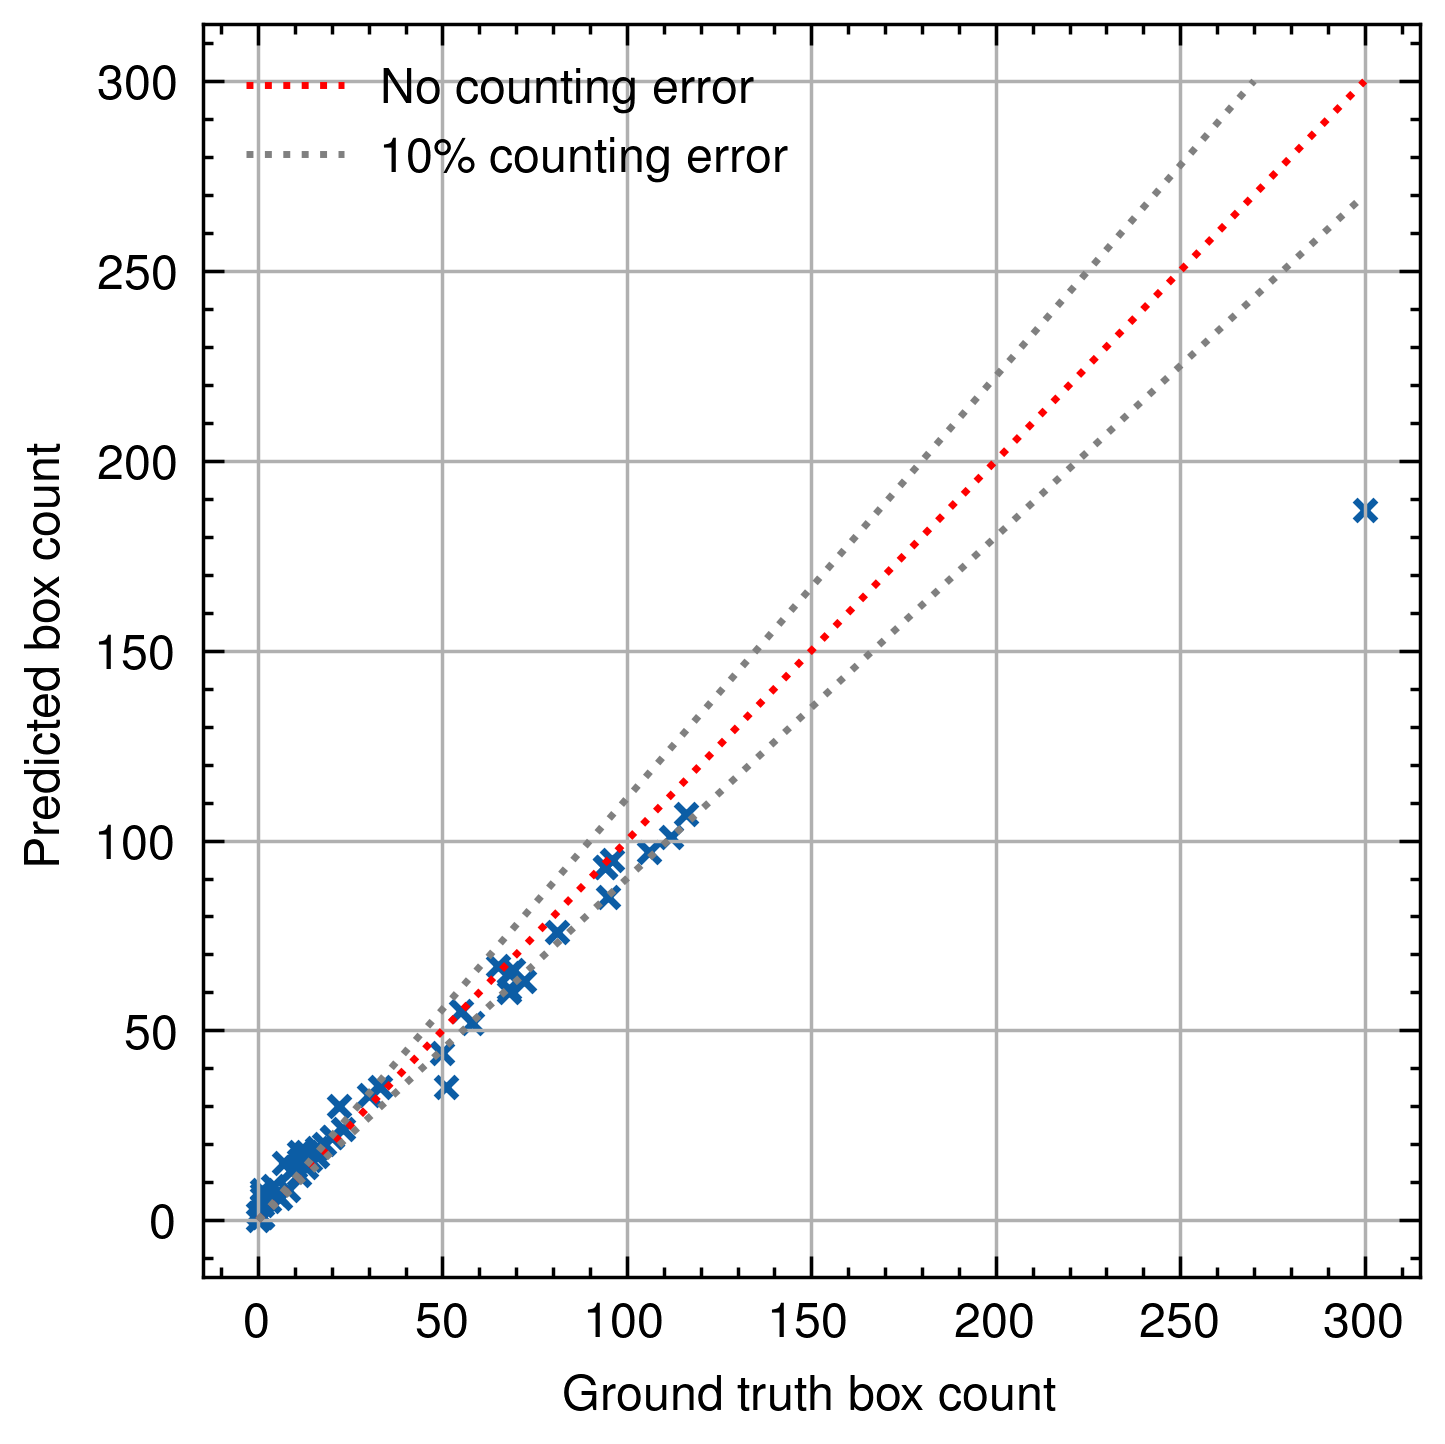
\includegraphics[width=\textwidth]{assets/chart_box_count}
         \caption{Chart showing counting error} 
         \label{fig:counting_test}
     \end{subfigure}
     \begin{subfigure}[b]{0.45\textwidth}
         \centering
         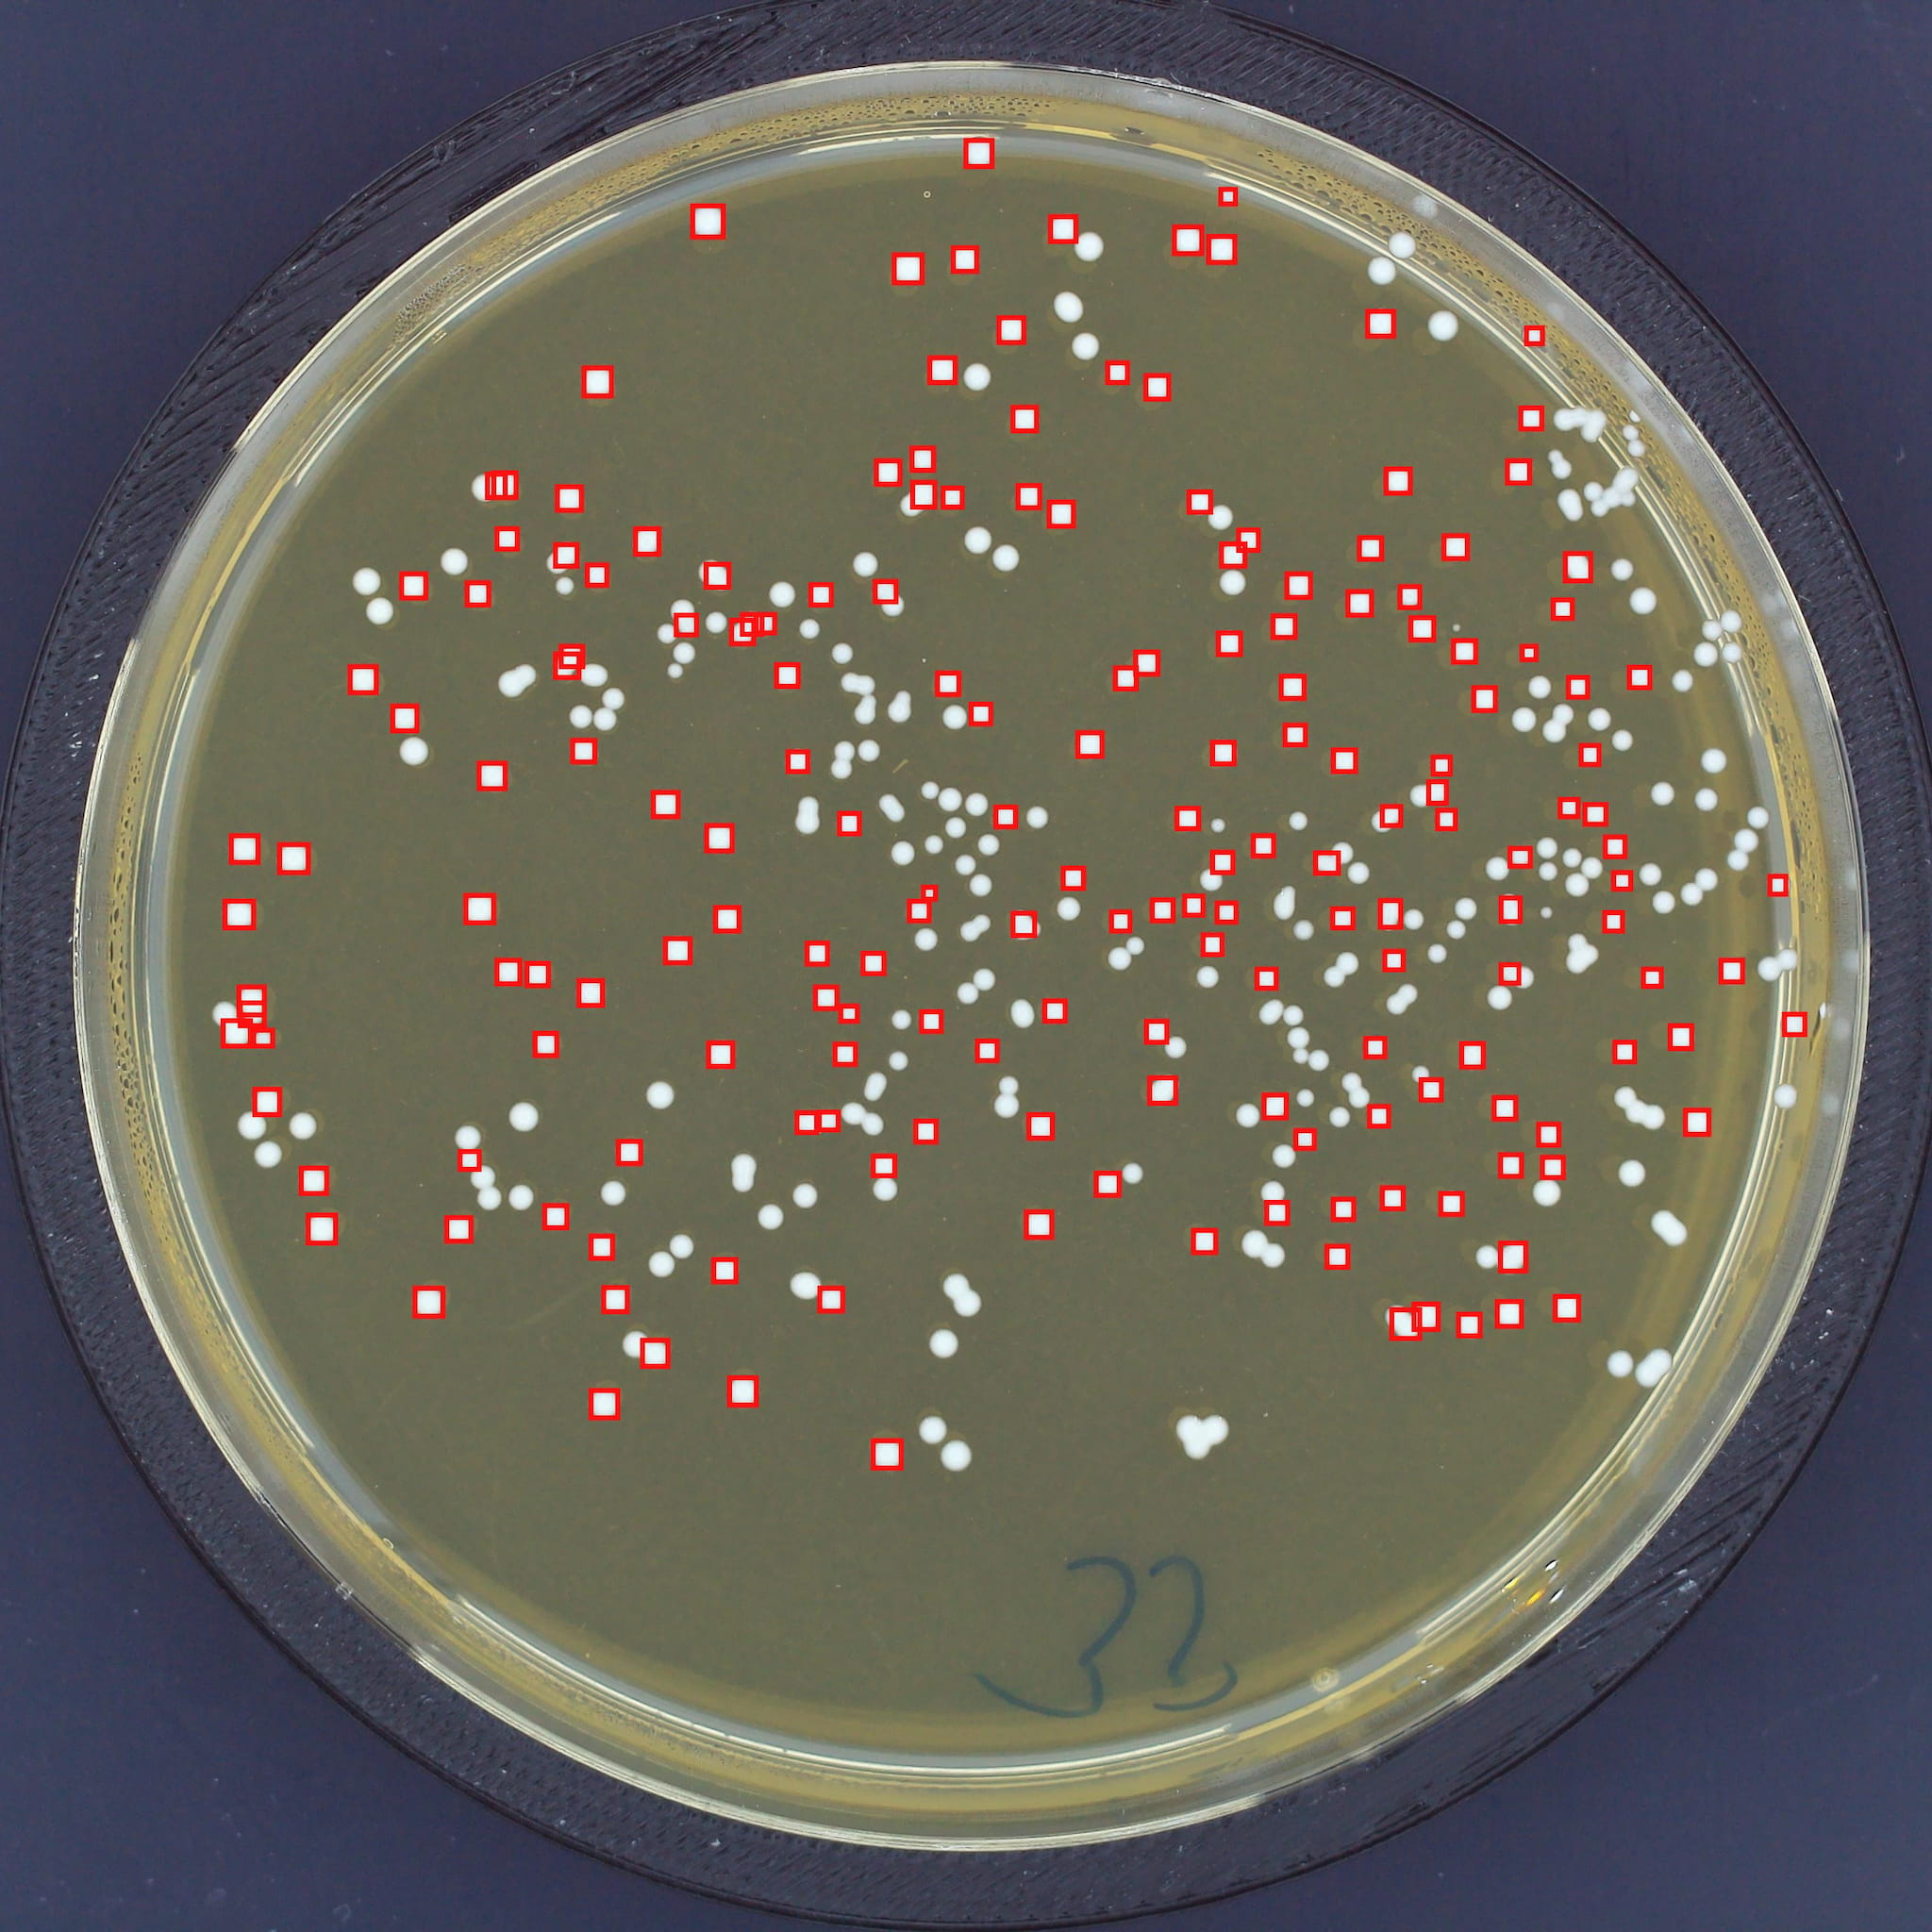
\includegraphics[width=\textwidth]{assets/test_set_outlier}
         \caption{Outlier image in test set}
         \label{fig:test_outlier}
     \end{subfigure}
     \caption{Counting performance on test set}
     \label{fig:test_counting_performance}
\end{figure}

\section{Qualitative Analysis}

\begin{figure}[hbt]
  \centering
  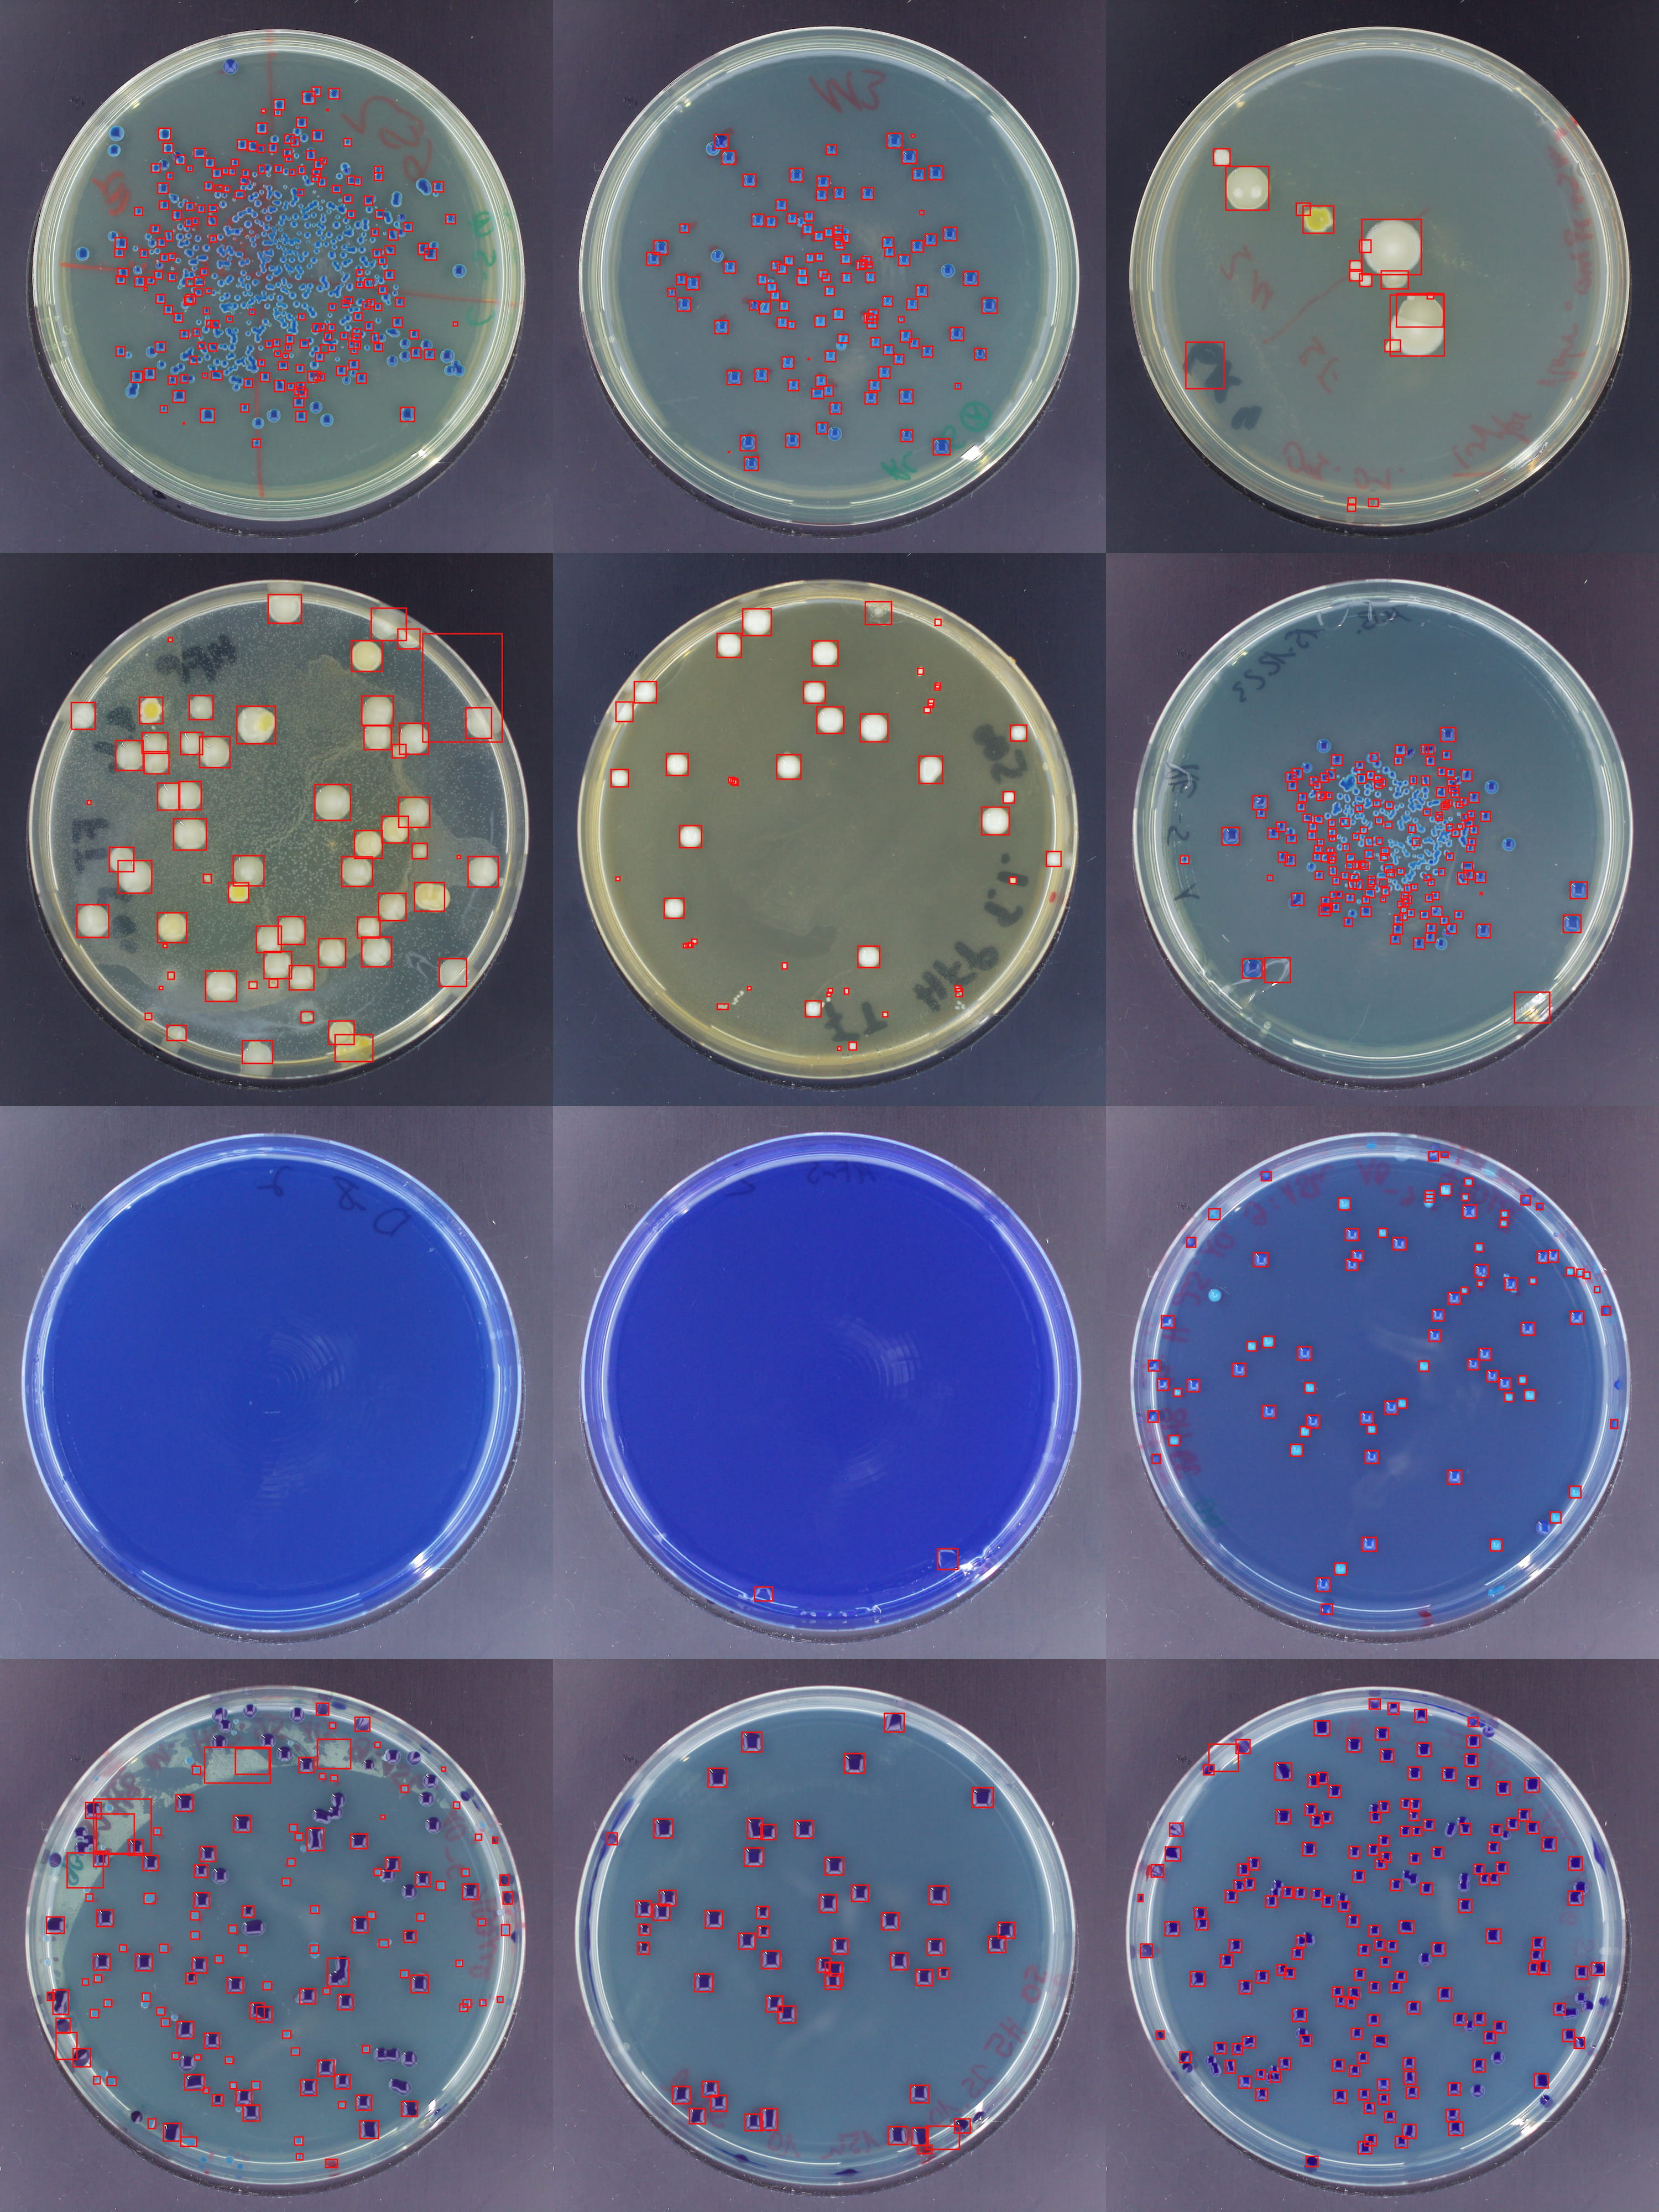
\includegraphics[width=\textwidth]{assets/chart_example_predictions}
  \caption{Examples of predictions for unlabeled images from the photobox dataset}
  \label{fig:example_predictions}
\end{figure}

To investigate the strengths and weaknesses of the model, all 276 unlabeled images from the photobox dataset were given to the model. Some of the results are shown in Figure \ref{fig:example_predictions}.

Generally, the model is able to precisely localize colonies when isolated. It generalizes beyond one style of image, having no problems finding colonies on different backgrounds or colonies of different shape and color.

As seen in the top right example of Figure \ref{fig:example_predictions}, the model can also segment colonies which have grown together a lot. It is also decent at detecting dishes as empty, with some false positive detections that have very low confidence scores. To combat this issue, confidence scores should be sharpened through more training (on more data) and the confidence threshold should be tuned.

It is really good at colony detection on images that contain only a single species with a light background, such as the bottom right images of Figure \ref{fig:example_predictions}. This is to be expected since a large part of the training dataset comprises similar images. The model seems to be fine for mixed species too, detecting two different types of species even if they differ in size, shape and color (see 9th image on Figure \ref{fig:example_predictions}).

The 4th image of Figure \ref{fig:example_predictions} shows that detection also goes beyond circle shapes. Even odd shapes can be detected and amorphous colonies, such as colonies that grow on the edge of the plate, are reliably detected as well.

The main problem of the model is detection in clusters of densely packed colonies, such as the top left image of Figure \ref{fig:example_predictions}. The boxes for these colonies are very close together and very small. This makes these images very inefficient to label, especially with the SAM-assisted labeling method described earlier, which is why they are rarely present in the photobox training data. Since they are very difficult to count, even for humans, some images of this type are marked as "uncountable" in the AGAR dataset. \cite{majchrowska2021agar}

As seen in the quantitative evaluation, the model has difficulties finding all colonies when there are a lot of them on the image. The photobox dataset is biased towards lower numbers of colonies per image, so this only makes sense. A more balanced dataset would most likely help combat this weakness.

Large false positive detections are also a minor issue, such as in the 4th image of Figure \ref{fig:example_predictions}. Since they usually have a very low confidence score, these should be fixable through post-processing and longer training schedules on more data.

\section{Discussion}

The precision of 92.9\% and recall of 87.3\% over the test set indicate strong performance for detecting colonies, however they leave room for improvements. The mean absolute error of 6.26 shows that the model cannot yet perfectly count the colonies in an image, but can approximate the number of colonies in an image pretty well.

This means the model can aid in counting and greatly reduce the time taken to count the colonies on a plate, since model errors are easy to spot. But if a precise count is needed, the model cannot yet be used in a fully automated fashion.

The impact of false positives on the detections for images with a low number of colonies on them is quite high. These false positives however mostly have a low confidence score. If the confidence score could be sharpened, these false positives would be sorted out easier. This could be improved by training longer on a larger dataset or finding reliable ways to augment the dataset.

For an average image of the test set, 78.1\% of predictions made on the image are correct and 21.9\% are false positives (precision). For recall, it correctly predicts 90.1\% of colonies and misses 9.9\%. Having a higher recall than precision is desirable here, since false positives are easier to dismiss than having to manually add missing bounding boxes.

The qualitative analysis matches the quantitative results, and shows which weaknesses hurt performance metrics. The weaknesses can be mostly traced back to imbalance in the training set, which is something that has to be improved for better general performance.

The difference in performance also brings up the question if specifically tuned models for different types of plates and species could yield better performance, since the model is very capable for certain types of images (spaced out colonies on clean backgrounds), while having trouble with other plates, which have artifacts on them, irregular shapes or just generally colonies of large area with odd shapes e.g. mold.
















